%% LaTeX Beamer presentation template (requires beamer package)
%% see http://bitbucket.org/rivanvx/beamer/wiki/Home
%% idea contributed by H. Turgut Uyar
%% template based on a template by Till Tantau
%% this template is still evolving - it might differ in future releases!

%% Template edited by Panagiotis Adamopoulos {padamopo}@stern.nyu.edu

\documentclass[aspectratio=169]{beamer}
 
\mode<presentation>
{
\usetheme{NYU}

\setbeamercovered{transparent}
}

\usepackage[english]{babel}
\usepackage[latin1]{inputenc}
\usepackage[scaled=.90]{helvet}
\usepackage{courier}
\usepackage[T1]{fontenc}
\usepackage{comment}
\usepackage{adjustbox}
%usepackage{appendixnumberbeamer}
\usepackage{amsmath}
\usepackage{bm}
\usepackage{pgfpages}
% citations
\usepackage{natbib}
\bibpunct{(}{)}{;}{a}{,}{,}
\def\citeapos#1{\citeauthor{#1}'s (\citeyear{#1})}
\renewcommand{\bibsection}{\subsubsection*{\bibname } }

\input{latex-math/basic-math.tex}
\input{latex-math/basic-ml.tex}
\input{latex-math/ml-svm.tex}

\newcommand{\zetai}{\zeta^{(i)}}

\title[]{\textbf{Exercise of Supervised Learning: \\ SVM Part 1}}

%\subtitle{}

% - Use the \inst{?} command only if the authors have different
%   affiliation.
%\author{F.~Author\inst{1} \and S.~Another\inst{2}}
\author{Yawei Li} 

% - Use the \inst command only if there are several affiliations.
% - Keep it simple, no one is interested in your street address.
\institute[LMU]
{
\\
  \texttt{yawei.li@stat.uni-muenchen.de}
}

\date{December 22, 2023}


% This is only inserted into the PDF information catalog. Can be left
% out.
\subject{Subject}



% If you have a file called "university-logo-filename.xxx", where xxx
% is a graphic format that can be processed by latex or pdflatex,
% resp., then you can add a logo as follows:

% \pgfdeclareimage[height=0.5cm]{university-logo}{university-logo-filename}
% \logo{\pgfuseimage{university-logo}}



% Delete this, if you do not want the table of contents to pop up at
% the beginning of each subsection:
%\AtBeginSubsection[]
%{
%\begin{frame}<beamer>
%\frametitle{Outline}
%\tableofcontents[currentsection,currentsubsection]
%\end{frame}
%}

% If you wish to uncover everything in a step-wise fashion, uncomment
% the following command:

%\beamerdefaultoverlayspecification{<+->}

\begin{document}



\begin{frame}[noframenumbering, plain]
\titlepage

\end{frame}

\begin{frame}{Exercise 1: Soft Margin Classifier}

The primal optimization problem for the two-class soft margin SVM classification is given by 
\begin{align*}
	\min_{\thetab, \theta_0, \zetai} & \frac{1}{2} ||\thetab||^2 + \sumin \zetai \\	
	\text{s.t.: }\quad & \yi (\thetab^T \xi + \theta_0) \geq 1 - \zetai, \\
	& \zetai \geq 0, \qquad \forall i= 1, \ldots, n.
\end{align*}

\begin{adjustbox}{valign=t}
	\begin{minipage}[t]{0.49\textwidth}
		(a) Add the decision boundary to the figure for $\thetabh = (1, 1)^T, \thetah_0 = -2$. (NB: This is the approximate optimum for $C = 10$).
	\end{minipage}
\end{adjustbox}
\hfill
\begin{adjustbox}{valign=t}
	\begin{minipage}{0.49\textwidth}
		\centering
		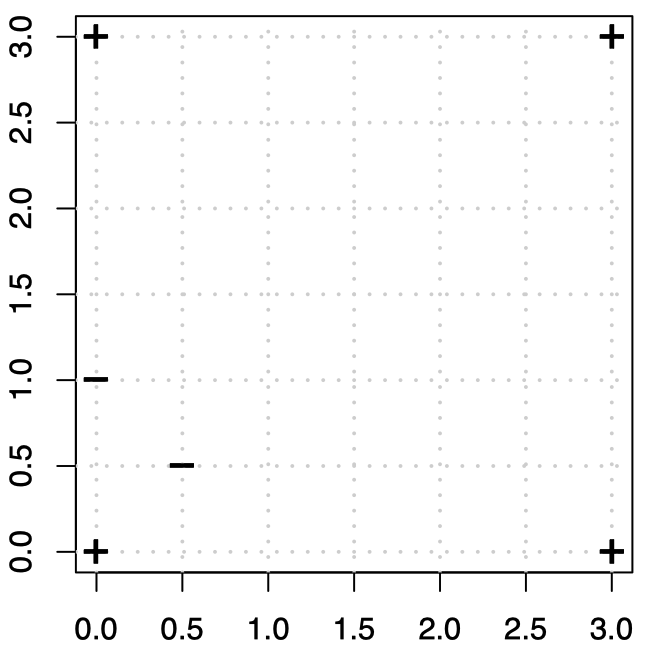
\includegraphics[width=0.6\columnwidth]{figures/ex_1_question.png}
	\end{minipage}

\end{adjustbox}

\end{frame}

\begin{frame}{Solution to Exercise 1 (a)}

\begin{columns}[T]
	\begin{column}[t]{0.49\textwidth}
		The hyperplane is given by:
		$$ \theta_1 x_1^{(i)} + \theta_2 x_2^{(i)} + \theta_0 = 0$$
		Plugging in the values for the $\theta$s and solving for $x_2$, we get the decision boundary:
		$$x_2 = - x_1 + 2$$
	\end{column}

	\hfill
	\begin{column}{0.49\textwidth}
		\centering
		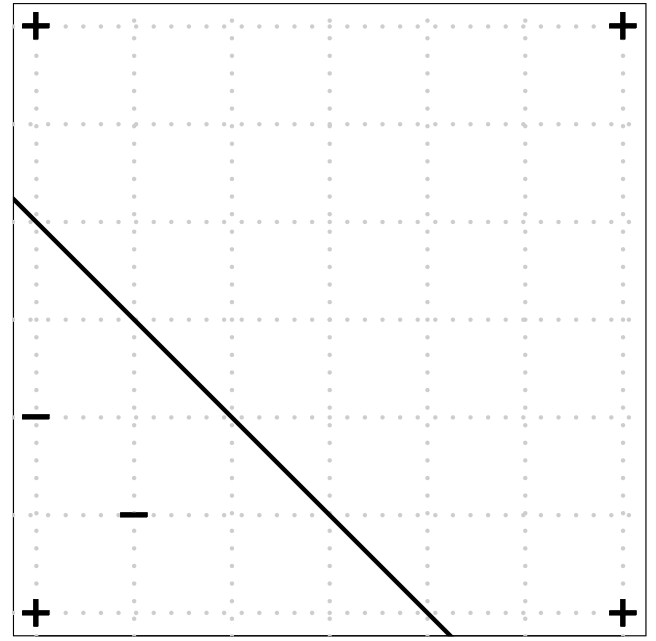
\includegraphics[width=0.6\columnwidth]{figures/ex_1_a_1.png}
		
		\textbf{Draw this figure on whiteboard.}
	\end{column}
\end{columns}
	
\end{frame}

\begin{frame}{Exercise 1 (b)}
	(b) Identify the coordinates of the support vector(s) and compute the values of their slack variable $\zetai$.
\end{frame}

\begin{frame}{Solution to Exercise 1 (b)}
	To determine which points are support vectors, we will use the constraint:
	\begin{align*}
		\yi (\xi \thetabh + \thetah_0) \geq 1 - \zetai 
	\end{align*}
	
	\begin{itemize}
		\item $(0,0)$: $1 (0 + 0 - 2) = -2 \geq 1 - \zeta^{(1)} \rightarrow \zeta^{(1)} \geq 3$, $\leadsto$ Support vector with slack variable $\zetai = 3$.
		\item $(0.5, 0.5)$: $-1 (0.5 + 0.5 - 2) = 1 \geq 1 - \zeta^{(2)} \rightarrow \zeta^{(2)} \geq 0$, $\leadsto$ Support vector with slack variable $\zetai = 0 $.
		\item $(0, 1)$: $ -1 (0 + 1 - 2) = 1 \geq 1 - \zeta^{(3)} \rightarrow \zeta^{(3)} \geq 0$, $\leadsto$ Support vector with slack variable $\zetai = 0$.
		\item $(0, 3)$: $ 1 (0 + 3 - 2) = 1 \geq 1 - \zeta^{(4)} \rightarrow \zeta^{(4)} \geq 0$, $\leadsto$ Support vector with slack variable $\zetai = 0$.
		\item $(3, 0)$: $ 1 (3 + 0 - 2) = 1 \geq 1 - \zeta^{(5)} \rightarrow \zeta^{(5)} \geq 0$, $\leadsto$ Support vector with slack variable $\zetai = 0$.
		\item $(3, 3)$: $ 1 (3 + 3 - 2) = 4 \geq 1 - \zeta^{(6)} \rightarrow \zeta^{(6)} \geq -3 $, $\leadsto$ \textbf{Not} a support vector.
	\end{itemize}
\end{frame}

\begin{frame}{Solution to Exercise 1 (b): Continued}
	\centering
	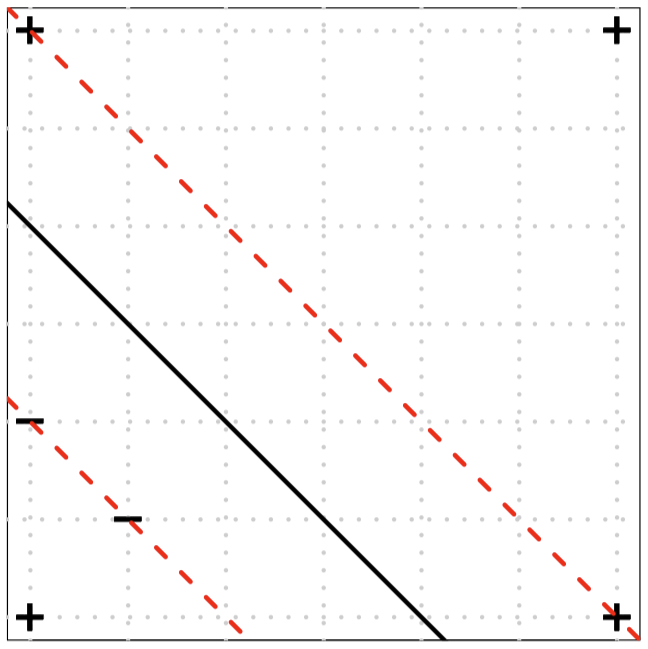
\includegraphics[width=0.5\textwidth]{figures/ex_1_b.png}
\end{frame}

\begin{frame}{Exercise 1 (c)}
	(c) Compute the Euclidean distance of the non-margin-violating support vector(s) to the decision boundary.
\end{frame}

\begin{frame}{Solution to Exercise 1 (c)}
	We can use $\xi = (0.5, 0.5)^T$:
	
	\begin{align*}
		d(f, \xi) = \frac{\yi f(\xi)}{||\thetab||_2} = \frac{-1 (0.5 + 0.5 - 2)}{\sqrt{2}} = \frac{1}{\sqrt{2}}
	\end{align*}
	The distance is the same for all non-margin-violating support vectors.
\end{frame}


\begin{frame}{Exercise 1 (d)}
	(d) What needs to be changed in the plot such that a hard margin SVM results into the same decision boundary?
\end{frame}

\begin{frame}{Solution to Exercise 1 (d)}
	Some alternatives are:
	\begin{itemize}
		\item Convert the $(0, 0)^T$ into a negative class.
		\item Move the $(0, 0)^T$ to $(2, 2)^T$.
		\item Delete $(0, 0)^T$.
	\end{itemize}
\end{frame}

\begin{frame}{Exercise 2: Optimization}
	Write your own stochastic subgradient descent routine to solve the soft-margin SVM in the primal formulation.
	
	\emph{Hints}:
	\begin{itemize}
		\item Use the regularized-empirical-risk-minimization formulation, i.e., an optimization criterion without constraints.
		\item No kernels, just a linear SVM.
		\item Compare your implementation with an existing implementation (e.g. \texttt{kernallab} in \texttt{R}. Are your results similar? Note that you might have to switch off the automatic data scaling in the already existing implementation.
	\end{itemize}
	
	\textbf{Solution: show the standard solution.}
\end{frame}

\end{document}
